
\documentclass[10pt]{article}
\usepackage[margin=0.62in]{geometry}
\usepackage[T1]{fontenc}
\usepackage{lmodern,microtype}
\usepackage{booktabs,tabularx,array,graphicx}
\usepackage{xcolor,amsmath,amssymb}
\usepackage{tikz}
\usetikzlibrary{arrows.meta,positioning,fit}
\usepackage{pgfplots}
\usepgfplotslibrary{groupplots}
\pgfplotsset{compat=1.18}
\usepackage[most]{tcolorbox}
\usepackage{enumitem}
\usepackage[hidelinks]{hyperref}

\definecolor{navy}{HTML}{17365D}
\definecolor{blue}{HTML}{2F75B5}
\definecolor{teal}{HTML}{1B998B}
\definecolor{orange}{HTML}{E67E22}
\definecolor{red}{HTML}{B03A2E}
\definecolor{green}{HTML}{2E7D32}
\definecolor{pale}{HTML}{F3F6FA}
\definecolor{rulegray}{HTML}{D5DBE3}
\setlength{\parindent}{0pt}
\setlength{\parskip}{3pt}
\setlist[itemize]{leftmargin=5mm,itemsep=2pt,topsep=2pt}
\renewcommand{\arraystretch}{1.10}
\newcommand{\NA}{\textemdash}
\newtcolorbox{infobox}[1][]{enhanced,boxrule=0.6pt,colback=pale,colframe=rulegray,
  arc=1.5mm,left=2mm,right=2mm,top=1.2mm,bottom=1.2mm,#1}
\newcommand{\metric}[1]{\textcolor{navy}{\bfseries #1}}

\begin{document}
\begin{center}
{\LARGE\bfseries\color{navy} 623 Direct-Action CNN vs. Offline Stride}\\[2pt]
{\small 623.xalancbmk\_s-700B \quad $\vert$ \quad seed 7 \quad $\vert$ \quad 25M measured instructions}\\[4pt]
\fcolorbox{green}{green!7}{\strut\bfseries PASS: fair-input and replay contracts}
\quad
\fcolorbox{red}{red!6}{\strut\bfseries No composite score; dimensions remain separate}
\end{center}

\begin{infobox}
\begin{tabularx}{\textwidth}{@{}>{\bfseries}lX@{}}
Primary comparison & Offline Stride actions versus independently generated CNN actions, replayed through the same transport and measured against the same no-prefetch baseline.\\
Shared external input & current PC and current cache-line address, in chronological order.\\
Neural history & two causal residual temporal-convolution layers; kernel 17, dilations 1 and 17, stride 1, receptive field 289 events.\\
Excluded at inference & Normal-prefetcher candidates, outputs, private tables/state, request budget/degree, future rows, and probability thresholds.  Teacher actions are labels only.\\
Run artifact & \texttt{623\_offline\_cnn\_stride\_variable\_delta\_free\_running\_v9\_seed7}.  ``PASS'' certifies the experiment contract; it does not certify useful neural behavior.\\
\end{tabularx}
\end{infobox}

\section*{1. What is measured}
\begin{center}
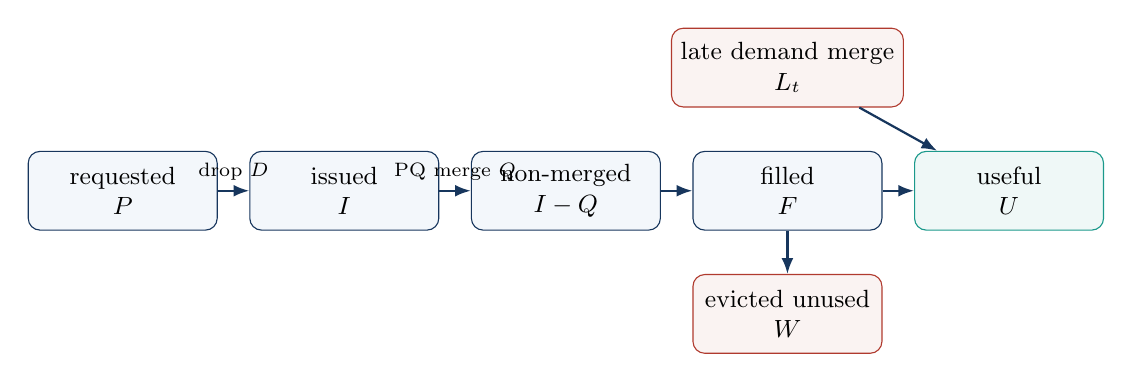
\begin{tikzpicture}[
  node distance=5.5mm and 4mm,
  every node/.style={font=\small},
  counter/.style={draw=navy,rounded corners=1.5mm,fill=blue!6,minimum width=24mm,minimum height=10mm,align=center},
  outcome/.style={draw=teal,rounded corners=1.5mm,fill=teal!7,minimum width=24mm,minimum height=10mm,align=center},
  bad/.style={draw=red,rounded corners=1.5mm,fill=red!6,minimum width=24mm,minimum height=10mm,align=center},
  arrow/.style={-{Latex[length=2mm]},thick,draw=navy}
]
\node[counter] (req) {requested\\$P$};
\node[counter,right=of req] (iss) {issued\\$I$};
\node[counter,right=of iss] (uniq) {non-merged\\$I-Q$};
\node[counter,right=of uniq] (fill) {filled\\$F$};
\node[outcome,right=of fill] (use) {useful\\$U$};
\node[bad,below=of fill] (waste) {evicted unused\\$W$};
\node[bad,above=of fill] (late) {late demand merge\\$L_t$};
\draw[arrow] (req)--node[above,font=\scriptsize]{drop $D$} (iss);
\draw[arrow] (iss)--node[above,font=\scriptsize]{PQ merge $Q$} (uniq);
\draw[arrow] (uniq)--(fill);
\draw[arrow] (fill)--(use);
\draw[arrow] (fill)--(waste);
\draw[arrow] (late)--(use);
\end{tikzpicture}
\end{center}

\begin{minipage}[t]{0.49\textwidth}
\begin{infobox}[title={\bfseries Outcome and reach}]
\[
 m=\frac{M}{N_L},\quad
 S=\frac{\mathrm{IPC}}{\mathrm{IPC}_0},\quad
 R_m=\frac{M_0-M}{M_0},\quad
 C=\frac{U}{M_0}.
\]
$N_L$ and $M$ are measured L2 loads and misses; subscript 0 denotes no prefetch.  $C$ is useful-prefetch coverage against no-prefetch misses, while $R_m$ is the observed miss reduction.  They are related but not interchangeable.
\end{infobox}
\end{minipage}\hfill
\begin{minipage}[t]{0.49\textwidth}
\begin{infobox}[title={\bfseries Accuracy, timeliness, and pressure}]
\[
 A=\frac{U}{I},\quad
 A_{\rm sel}=\frac{U}{I-Q},\quad
 T=\frac{U}{U+L_t},\quad
 \rho=\frac{P}{N_L}.
\]
$A$ counts every issued attempt.  The project-defined $A_{\rm sel}$ removes PQ-merged duplicates from the denominator.  It is not a pollution metric. $T$ asks whether useful requests arrived before demand; $\rho$ exposes request pressure.
\end{infobox}
\end{minipage}

\begin{infobox}[title={\bfseries Exact interpretation boundaries}]
The formulas above are taken from the experiment analyzers and recomputed from
the simulator counters, not inferred from CSV names.  A source audit of
\texttt{src/cache.cc} confirms the lifecycle: $U$ increments on the first read
hit to a prefetched line and clears its prefetch bit; $W$ increments when a
still-prefetched, unused line is replaced; $F$ increments when a prefetch is
filled; $L_t$ increments when demand merges into an in-flight prefetch; and
$Q$ increments for a duplicate in the prefetch queue.  When a denominator is
zero, the ratio is reported as \NA; a safe-divide value of zero in JSON is not
treated as a valid 0\% accuracy/timeliness result.  We also report
$U/M$, $Q/I$, $D/P$, $F/(I-Q)$, $L_t/I$, $W/I$, and resolved-fill
utility $U/(U+W)$.  These labels state the numerator and denominator
explicitly: $U/M$ can exceed one and is not coverage, while $F/(I-Q)$ is an
issue-to-fill reach ratio rather than usefulness.
Hennessy and Patterson motivate these separate dimensions: bad prefetches can
displace useful blocks and consume bandwidth, while useful prefetches must
arrive in time and avoid excessive outstanding work.\footnote{J. L. Hennessy
and D. A. Patterson, \emph{Computer Architecture: A Quantitative Approach},
7th ed., Sec.~2.3, pp.~127--129; Exercise~2.3, p.~160.}
No direct harmful-victim/re-reference counter exists here.  $W$ and request
pressure indicate risk, but neither proves cache pollution; consequently
$1-A_{\rm sel}$ is not reported as pollution and no aggregate score is used.
\end{infobox}

\section*{2. Cache outcomes}
\begin{center}\scriptsize
\resizebox{\textwidth}{!}{%
\begin{tabular}{@{}lrrrrrrrr@{}}
\toprule
Method & params & cycles & IPC & speedup & L2 loads & L2 misses & miss rate & miss reduction \\
\midrule
No prefetch & -- & 70.780M & 0.35321 & 1.0000 & 1,218,494 & 450,350 & 36.96\% & 0.00\% \\
Offline Stride & -- & 70.742M & 0.35340 & 1.0005 & 1,218,495 & 448,288 & 36.79\% & 0.46\% \\
Live Stride (context) & -- & 70.742M & 0.35340 & 1.0005 & 1,218,495 & 448,287 & 36.79\% & 0.46\% \\
CNN c7 & 2,953 & 70.775M & 0.35323 & 1.0001 & 1,218,494 & 450,091 & 36.94\% & 0.06\% \\
CNN c15 & 10,873 & 70.769M & 0.35326 & 1.0001 & 1,218,494 & 449,771 & 36.91\% & 0.13\% \\
CNN c24 & 25,597 & 70.756M & 0.35333 & 1.0003 & 1,218,494 & 445,895 & 36.59\% & 0.99\% \\
\bottomrule
\end{tabular}}
\end{center}

\begin{center}
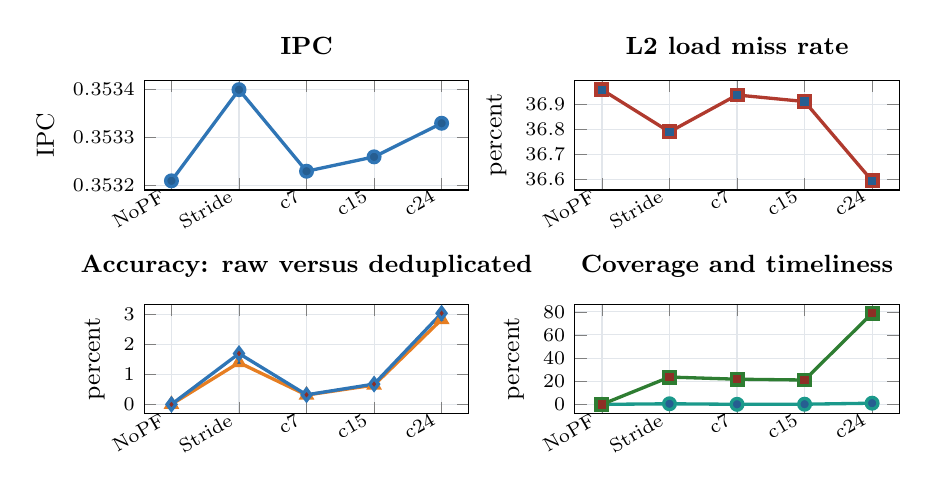
\begin{tikzpicture}
\begin{groupplot}[
  group style={group size=2 by 2,horizontal sep=1.35cm,vertical sep=1.45cm},
  width=0.47\textwidth,height=0.245\textwidth,
  grid=major,grid style={rulegray!70},
  tick label style={font=\scriptsize},label style={font=\small},title style={font=\small\bfseries},
  xtick={0,1,2,3,4},xticklabels={{NoPF},{Stride},{c7},{c15},{c24}},
  x tick label style={rotate=30,anchor=east},
  every axis plot/.append style={very thick,mark size=2.1pt}
]
\nextgroupplot[title={IPC},ylabel={IPC},scaled y ticks=false,
  yticklabel style={/pgf/number format/fixed,/pgf/number format/precision=5}]
\addplot+[color=blue,mark=*] coordinates {(0,0.35321000) (1,0.35340000) (2,0.35323000) (3,0.35326000) (4,0.35333000)};
\nextgroupplot[title={L2 load miss rate},ylabel={percent},scaled y ticks=false]
\addplot+[color=red,mark=square*] coordinates {(0,36.95955827) (1,36.79030279) (2,36.93830253) (3,36.91204060) (4,36.59394301)};
\nextgroupplot[title={Accuracy: raw versus deduplicated},ylabel={percent},scaled y ticks=false]
\addplot+[color=orange,mark=triangle*] coordinates {(0,0) (1,1.39153882) (2,0.31120695) (3,0.64295863) (4,2.82853040)};
\addplot+[color=blue,mark=diamond*] coordinates {(0,0) (1,1.69425697) (2,0.31930924) (3,0.67604604) (4,3.03555653)};
\nextgroupplot[title={Coverage and timeliness},ylabel={percent},scaled y ticks=false]
\addplot+[color=teal,mark=*] coordinates {(0,0.00000000) (1,0.51337848) (2,0.05928722) (3,0.13966915) (4,1.01476629)};
\addplot+[color=green,mark=square*] coordinates {(0,0) (1,23.59665238) (2,21.74267101) (3,21.03678930) (4,78.73880083)};
\end{groupplot}
\end{tikzpicture}

\vspace{1mm}
{\footnotesize
\textcolor{orange}{Orange triangles}: raw accuracy $A=U/I$;\quad
\textcolor{blue}{blue diamonds}: selected accuracy $A_{\rm sel}=U/(I-Q)$;\quad
\textcolor{teal}{teal circles}: coverage $C$;\quad
\textcolor{green}{green squares}: timeliness $T$.\\
Series labels are outside every plot and title.  No-action points are drawn at
zero for visibility; their zero-denominator accuracy/timeliness entries remain
\NA\ in the tables.}
\end{center}

\section*{3. Quality and traffic---kept separate}
\begin{center}\scriptsize
\resizebox{\textwidth}{!}{%
\begin{tabular}{@{}lrrrrr@{}}
\toprule
Method & raw accuracy $U/I$ & selected accuracy $U/(I-Q)$ & coverage $U/M_0$ & useful/self-miss $U/M$ & timeliness $U/(U+L_t)$ \\
\midrule
Offline Stride & 1.39\% & 1.69\% & 0.51\% & 0.005 & 23.60\% \\
CNN c7 & 0.31\% & 0.32\% & 0.06\% & 0.001 & 21.74\% \\
CNN c15 & 0.64\% & 0.68\% & 0.14\% & 0.001 & 21.04\% \\
CNN c24 & 2.83\% & 3.04\% & 1.01\% & 0.010 & 78.74\% \\
\bottomrule
\end{tabular}}
\end{center}

\begin{center}\scriptsize
\resizebox{\textwidth}{!}{%
\begin{tabular}{@{}lrrrrrrr@{}}
\toprule
Method & request/L2 load $P/N_L$ & merge/issued $Q/I$ & drop/request $D/P$ & fill/non-merged $F/(I-Q)$ & late/issued $L_t/I$ & useless/issued $W/I$ & resolved-fill utility $U/(U+W)$ \\
\midrule
Offline Stride & 0.136 & 17.867\% & 0.000\% & 1.781\% & 4.506\% & 0.070\% & 95.18\% \\
CNN c7 & 0.070 & 2.537\% & 0.000\% & 0.319\% & 1.120\% & 0.000\% & 100.00\% \\
CNN c15 & 0.080 & 4.894\% & 0.000\% & 0.676\% & 2.413\% & 0.000\% & 100.00\% \\
CNN c24 & 0.133 & 6.820\% & 0.000\% & 3.138\% & 0.764\% & 0.093\% & 96.80\% \\
\bottomrule
\end{tabular}}
\end{center}

\begin{center}\scriptsize
\resizebox{\textwidth}{!}{%
\begin{tabular}{@{}lrrrrrrrrr@{}}
\toprule
Method & requested $P$ & dropped $D$ & issued $I$ & PQ merged $Q$ & $I-Q$ & filled $F$ & useful $U$ & useless $W$ & late $L_t$ \\
\midrule
Offline Stride & 166,147 & 0 & 166,147 & 29,686 & 136,461 & 2,431 & 2,312 & 117 & 7,486 \\
CNN c7 & 85,795 & 0 & 85,795 & 2,177 & 83,618 & 267 & 267 & 0 & 961 \\
CNN c15 & 97,829 & 0 & 97,829 & 4,788 & 93,041 & 629 & 629 & 0 & 2,361 \\
CNN c24 & 161,568 & 0 & 161,568 & 11,019 & 150,549 & 4,724 & 4,570 & 151 & 1,234 \\
\bottomrule
\end{tabular}}
\end{center}

\begin{infobox}[title={\bfseries Why raw and selected accuracy can disagree}]
PQ-merged requests remain in $I$ but are removed from $I-Q$.  Therefore
$A_{\rm sel}$ can rise sharply when duplicate merging is high even if $U$ does
not rise.  The lifecycle table is the denominator audit: selected accuracy is
never interpreted without raw accuracy, merge count, coverage, miss rate, and
IPC.
\end{infobox}

\section*{4. Data-supported insights}
\begin{infobox}[fontupper=\small]
\begin{itemize}[itemsep=1pt,topsep=1pt]
\item c24 is the only material CNN point: miss rate 36.594\% versus 36.790\% for offline Stride, coverage 1.015\% versus 0.513\%, and timeliness 78.74\% versus 23.60\%.
\item Despite those better cache ratios, c24 IPC is 0.35333 versus 0.35340 (a -0.02\% gap).  The effect is extremely small on this single trace/seed, so cache metrics and IPC must remain separate outcomes.
\item c7 and c15 have very low fill and coverage.  Capacity helps here, but no tested CNN beats the offline Stride IPC reference.
\end{itemize}
\end{infobox}

\section*{5. Event-log audit and 602/623 schema difference}
\begin{center}\scriptsize
\resizebox{\textwidth}{!}{%
\begin{tabular}{@{}lrrrrrrrrrr@{}}
\toprule
Method & demand & demand miss & PF event & accepted & duplicate & action L2 & action LLC & fill feedback & useful-demand hit & late-demand miss \\
\midrule
Offline Stride & 1,218,495 & 448,288 & 166,147 & 166,147 & 29,686 & 166,147 & 0 & -- & 2,119 & 7,486 \\
CNN c7 & 1,218,494 & 450,091 & 85,795 & 85,795 & 2,177 & 85,795 & 0 & -- & 259 & 961 \\
CNN c15 & 1,218,494 & 449,771 & 97,829 & 97,829 & 4,788 & 97,829 & 0 & -- & 582 & 2,361 \\
CNN c24 & 1,218,494 & 445,895 & 161,568 & 161,568 & 11,019 & 161,568 & 0 & -- & 4,407 & 1,233 \\
\bottomrule
\end{tabular}}
\end{center}

\begin{tabularx}{\textwidth}{@{}>{\bfseries}lXX@{}}
\toprule
Evidence & 602 logger/results & 623 logger/results \\
\midrule
Simulator final counters & IPC, loads/misses, requested/dropped/issued/merged/filled/useful/useless/late are present in the raw logs. & Same counters are copied into the JSON/CSV summary.\\
Demand-event attribution & demand, miss, PF request, useful-demand hit, and late-demand miss. & Same core fields plus accepted, duplicate, fill-level, and (SPP) fill-feedback counts.\\
Teacher imitation & not part of the cache-effect summary. & SPP only: precision/recall/F1 and count/fill diagnostics; these are model diagnostics, not cache metrics.\\
Direct pollution & Not measured: the schema does not identify a useful victim displaced by a prefetch and later re-referenced. & Not measured; the same limitation applies.\\
\bottomrule
\end{tabularx}

\begin{infobox}[title={\bfseries Replay decision}]
For 602, the apparently missing 623 metrics are a \emph{summary-schema}
difference: the required simulator counters already exist in the archived raw
logs and are used above.  No 602 replay is needed for miss rate, raw/selected
accuracy, coverage, timeliness, request pressure, merges, fills, useful,
useless, or late counts.  A new instrumented replay is needed only if the
presentation requires direct harmful-eviction pollution or the newer
accepted/fill-level event audit.
\end{infobox}

{\footnotesize The main formulas use the simulator-final counters exactly as
the analyzers do.  The event-log counts above are an independent attribution
audit and are never substituted into $A$, $A_{\rm sel}$, $C$, or $T$.}



\end{document}
